%!TEX root = ../template.tex
%%%%%%%%%%%%%%%%%%%%%%%%%%%%%%%%%%%%%%%%%%%%%%%%%%%%%%%%%%%%%%%%%%%%
%% chapter4.tex
%% NOVA thesis document file
%%
%% Chapter with lots of dummy text
%%%%%%%%%%%%%%%%%%%%%%%%%%%%%%%%%%%%%%%%%%%%%%%%%%%%%%%%%%%%%%%%%%%%

\typeout{NT FILE chapter4.tex}%

\chapter{Proposed Work}
\label{cha:proposed_work}

%\section{Requirements and Proposed Methodology}
\section{Requirements}

\subsection*{Interactive Map}
\begin{itemize}
    \item \textbf{Map Zoom \& Navigation:} Users can pan, zoom, and explore different locations.
    \item \textbf{Perspective Switching:} Toggle between top-down and profile views for better spatial understanding.
    \item \textbf{Geospatial Data Integration:} Include \gls{GIS} layers combining excavation findings, a historical map, and overlay a \textit{.tif} map illustration.
    \item \textbf{Layer Toggle:} Toggle visibility of layers, such as excavation campaigns or glass artifacts.
    \item \textbf{Parallel Objects:} Link parallel excavation findings/museum(possibly in the object pop-up in the map).
\end{itemize}

\subsection*{\gls{3D} Models \& Interaction}
\begin{itemize}
    \item \textbf{Artifact Interaction:} Allows users to virtually manipulate (rotate, zoom) the glass artifact models, as well as apply different textures.
    \item \textbf{Contextual Overlay:} Display descriptive metadata about the artifact, such as its origin, period, and historical usage.
    \item \textbf{Reconstructed Models:} Showcase how artifacts would look originally(having in consideration characteristics such as: colourless glass, archeological drawings).
    \item \textbf{3D Models Integration:} The user can zoom the map to visualize the perspective of a specific \gls{3D} model.
    %select a position to visualize the perspective of their 3D model.
\end{itemize}

\subsection*{Repository}
\begin{itemize}
    \item \textbf{Document Upload/Download:} Allow contributors to upload images, videos or excavation reports of the archeological intervention.
    \item \textbf{Search and Filter Features:} Users can search and filter based on some fields, such as time period, shape, and provenance.
    \item \textbf{Digital Preservation:} Utilization of open, and standard formats to ensure a long-term resource access.
\end{itemize}


\subsection*{\gls{AR} Integration}
\begin{itemize}
    \item \textbf{Immersive Experience:} Augmented reality allows users to virtually augment a tomb visit, enabling interaction with glass artifacts.
    \item \textbf{Device Accessibility:} Primarily user-friendly and enabling haptic interaction, while supporting \gls{AR} glasses as an emerging display option.
    \item \textbf{Localization \& Wayfinding:} 
    \begin{itemize}
        \item \textbf{\gls{POI}:} Use colors, text, visual markers, or direction arrows to emphasize and guide users to historically significant locations.
    \end{itemize}
   % \item \textbf{Multilingual Support:} Provide language options to ensure accessibility for an international audience.
\end{itemize}



\section{Development Technologies and Tools}
\label{sec:technologies}


\subsection{Frontend Technologies}
\label{sec:frontend}

\subsection{Backend Technologies}
\label{sec:backend} 

\subsection{VR Tools}
\label{sec:vr_tools} 


\subsection{Photogrammetry Tools}
\label{sec:photogrammetry_tool} 

The software that will be used to process digital images and generate \gls{3D} object models is \textit{Agisoft Metashape}\footnote{https://www.agisoft.com/}.
This software performs photogrammetric processing of digital images to generate \gls{3D} spatial data, which can be applied in various fields such as \gls{GIS} applications, \gls{CH} documentation, visual effects production, and indirect measurements of objects of diverse scales. 
By stitching together photographs, \textit{Agisoft Metashape} captures the geometry, texture, and visual appearance of physical objects or environments.
\subsection{GIS Tools}
\label{sec:gis} 


\section{System Architecture}
\label{sec:architecture}


\begin{figure}[h!]
    \centering
    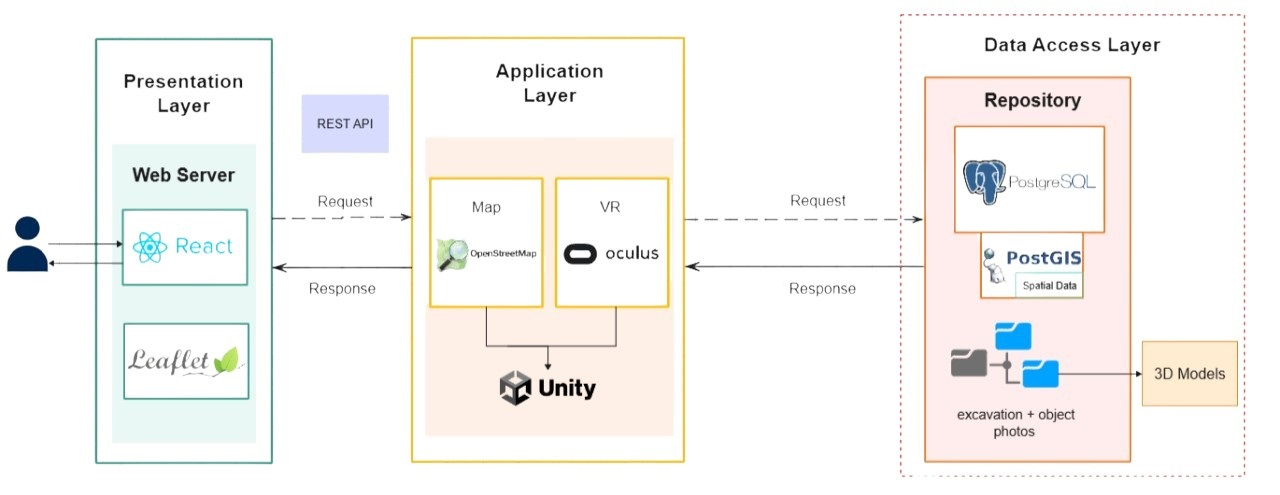
\includegraphics[width=1.0\linewidth]{System Architecture-Photoroom_Right}
    \caption{System Architecture Overview}
    \label{fig:architecture}
  \end{figure}
  \FloatBarrier


\section{Data Repository}
\label{sec:data_repository}


\section{Usability Tests}
\label{sec:usability_tests}



\section{Previous Work}
\label{sec:previous_work}

During my internship, I developed a platform using React and TailwindCSS for the web layer, with C\# and ASP.NET for the application layer, and MongoDB for data storage. Communication between these three components was handled through direct requests to the web server, which forwarded CRUD operations and interacted with the database.  
Additionally, the Database Systems and Cloud Computation Systems master's course provided me with hands-on experience in various storage methodologies and introduced me to different technologies and alternative solutions for data management.

\subsection{Geographic Information System}
\label{sec:gis_previous} 

To deepen my expertise in \gls{GIS}, I enrolled in the master's course \textit{Web Geográfica}, taught by my thesis adviser, Armanda Rodrigues. During this course, I developed a Web \gls{3D} application designed to provide an interactive map for visualizing and analyzing demographic data, key infrastructure locations, and other notable European datasets. Although this project did not focus on archaeological data, it introduced me to and enriched my understanding of GIS concepts, map interaction, and geospatial analysis while exposing me to new technologies.

The application leveraged PostGIS\footnote{https://postgis.net/}, a PostgreSQL extension, which is widely used for spatial data storage, geometry processing, and querying geospatial data efficiently.
Additionally, used frameworks like Leaflet\footnote{https://leafletjs.com/}, an open-source JavaScript library that facilitates the creation of mobile-friendly interactive maps. Leaflet offers a wide array of plugins that improve the usability and simplicity of the application. For the base map, \gls{OSM}\footnote{https://www.openstreetmap.org/} was integrated, offering a customizable and versatile visualization. This project serves as a preparatory stage for my thesis, specifically for the \gls{GIS} component, in which I will develop an interactive map of the Tróia site.

\subsection{Photogrammetry}
\label{sec:photogrammetry_previous} 

A photogrammetric simulation was conducted using the \textit{Agisoft Metashape} environment. A total of 143 images were collected during the excavation campaign by the restoration department of NOVA, for analysis. 
Based on these images, a \gls{3D} model was generated and subsequently imported into the \textit{Sketchfab} viewer for intuitive interaction, as shown in Figure~\ref{fig:model3}.


\begin{figure}[h]
    \centering
    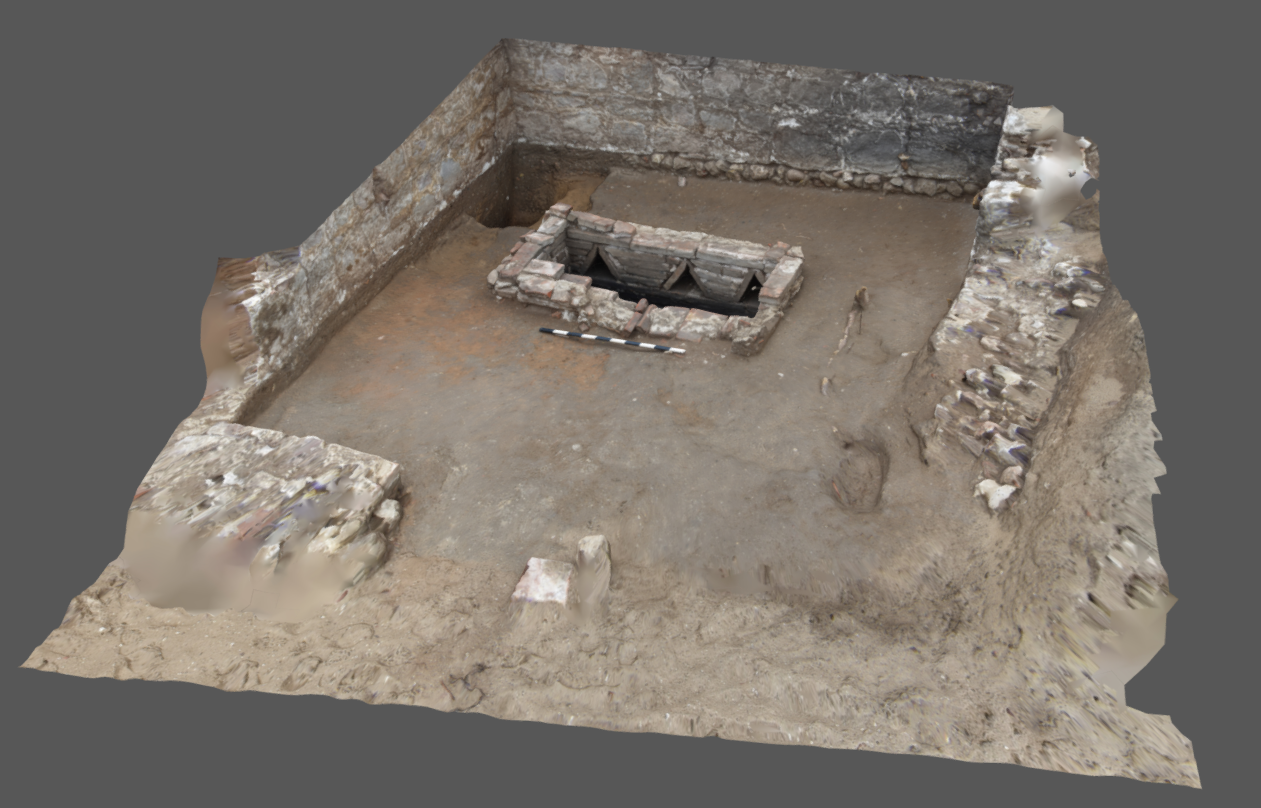
\includegraphics[width=0.7\textwidth]{model3}
    \caption{\gls{3D} model imported into Sketchfab for visualization.}
    \label{fig:model3}
\end{figure}


\subsection{Unity}
\label{sec:unity} 



\begin{figure}[h]
    \centering
    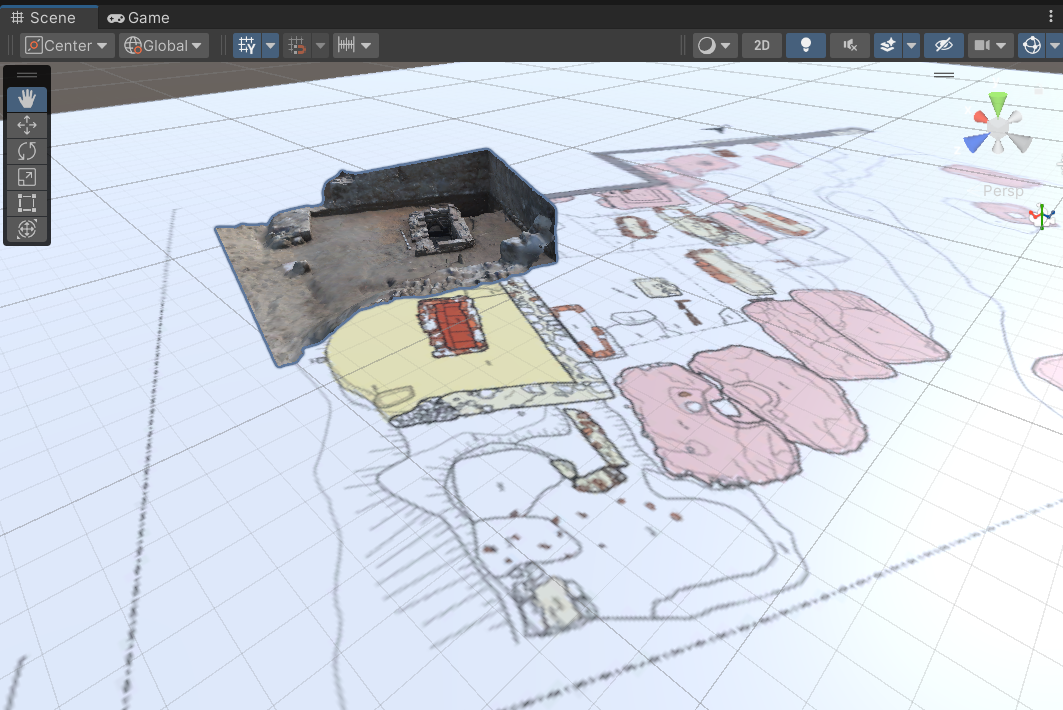
\includegraphics[width=0.7\textwidth]{overlay_test}
    \caption{Overlay \gls{3D} excavation model with a map representation.}
    \label{fig:overlay}
\end{figure}


%Insights from the Research Unit VICARTE